\chapter{Regression: Zahlenwerte vorhersagen}
\label{chap:regression}

\begin{myremark}[Algorithmusart in diesem Kapitel]
Funktionsart: \textbf{Regression}. \\
Umsetzungsart: \textbf{selbstlernend}.
\end{myremark}

\section{Lineare Regression für Regression}

\begin{mydefinition}
Die \textbf{lineare Regression} sagt einen Zahlenwert \(y\) auf Basis von Merkmalen \(x_1, x_2, \ldots\)
vorher. Ein einfaches Modell lautet:
\[
y = a_0 + a_1x_1 + a_2x_2
\]
\end{mydefinition}

\begin{figure}[H]
    \centering
    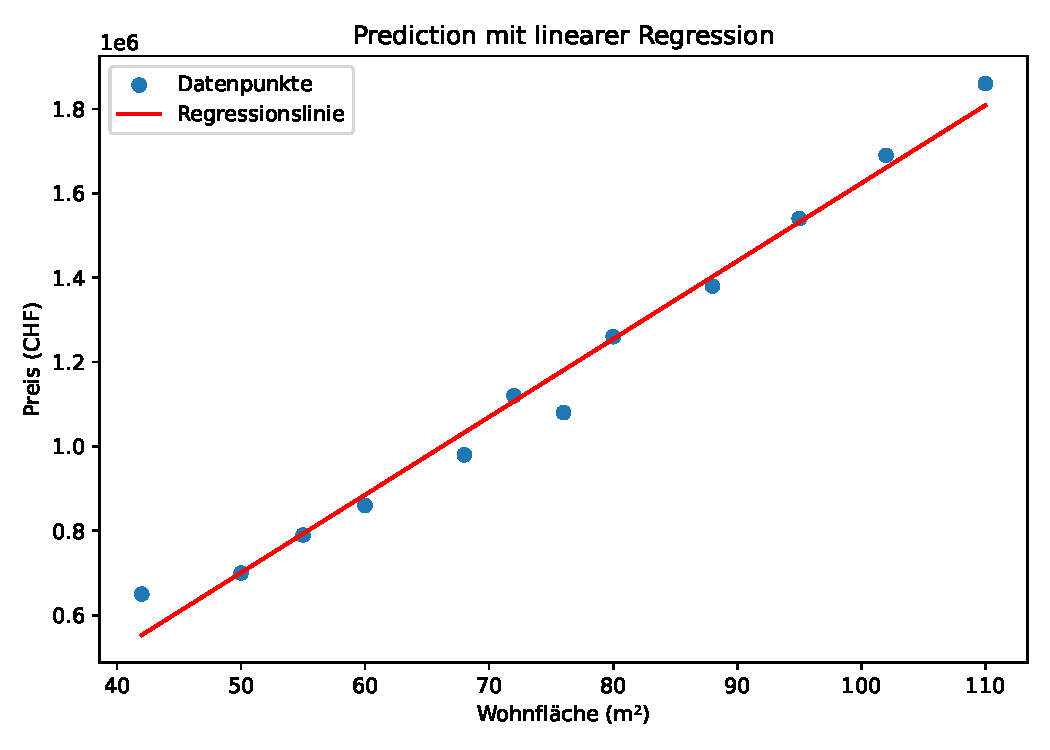
\includegraphics[width=0.75\textwidth]{Grundlagen_Info/10_KI_und_Algorithmen/Figures/regression_prediction.pdf}
    \caption{Beispiel einer Regression mit linearer Regression}
    \label{fig:reg-pred-15}
\end{figure}

\begin{myexercise}[Interpretation]
In \cref{fig:reg-pred-15} steigt die Vorhersage mit zunehmender Wohnfläche.
\begin{enumerate}
    \item Was bedeutet eine positive Steigung inhaltlich?
    \item Nennen Sie zwei weitere Merkmale, die den Preis beeinflussen könnten.
\end{enumerate}
\end{myexercise}

\begin{myexercise}[Fehlermasse]
Nennen und erklären Sie kurz:
\begin{itemize}
    \item MAE (Mean Absolute Error)
    \item RMSE (Root Mean Squared Error)
\end{itemize}
Welches Mass bestraft grosse Fehler stärker?
\begin{myanswer}
RMSE bestraft grosse Fehler stärker, weil die Fehler zuerst quadriert werden.
\end{myanswer}
\end{myexercise}

\begin{myremark}[Notebook]
Praktische Umsetzung inkl. Übungen:
\href{\notebookbaseurl05_Regression_Prediction.ipynb}{\texttt{05\_Regression.ipynb}}
\end{myremark}
